\documentclass[eng,printmode,oneside]{mgr}
\usepackage[MeX]{polski}
\usepackage[utf8]{inputenc}
\usepackage[T1]{fontenc} 
\usepackage{graphicx}
\usepackage{subfigure}
\usepackage{psfrag}
\usepackage{amsmath}
\usepackage{amsfonts}
%\usepackage{supertabular}
\usepackage{array}
\usepackage{tabularx}
\usepackage{hhline}
\usepackage{rev}
%\usepackage{framed}
\usepackage{color}
\usepackage{url}
%\usepackage[notref]{showkeys}
%\usepackage{showlabels}
\usepackage{float}
%\usepackage{tikz}
\usepackage{enumitem} 
\usepackage{graphicx}       
\usepackage{rotating}       % pakiet umożliwiający obracanie rysunków
\usepackage{subfigure}      % pakiet umożliwiający tworzenie podrysunków
\usepackage{epic}           
\usepackage{listings}       % pakiet dedykowany zrodlom programow
\usepackage{verbatim}       % pakiet dedykowany rozmaitym wydrukom tekstowym
\usepackage{amssymb}        % pakiet z rozmaitymi symbolami matematycznymi
\usepackage{amsmath}        % pakiet z rozmaitymi środowiskami matematycznymi
\usepackage[polish]{babel}  % pakiet lokalizujący dokument w języku polskim
\usepackage[OT4]{fontenc}
\usepackage[utf8]{inputenc}
\usepackage{bm}
\usepackage{gensymb}
\usepackage{booktabs}
\usepackage{epstopdf}
\usepackage{amssymb}
\usepackage[utf8]{inputenc}
\usepackage{amsmath}
\usepackage{amsfonts}
\usepackage{amssymb}
\usepackage{graphics}
\usepackage[]{algorithmic} %pseudocode
\usepackage[]{algorithm2e} %pseudocode
\usepackage{float}
\usepackage{csquotes}
\usepackage{epsfig}
%\usepackage{hyperref}
\usepackage{wrapfig} 
\reviewer{dypl}{0.2}{0.2}{0.67}
\reviewer{prof}{0.2}{0.6}{0.2}
\def\bp{\begin{review}[prof]}
\def\ep{\end{review}}
\def\bdypl{\begin{review}[dypl]}
\def\edypl{\end{review}}
\newcommand{\R}{I\!\!R} 
\newtheorem{theorem}{Twierdzenie}[section] 
\newcommand\numberthis{\addtocounter{equation}{1}\tag{\theequation}}
\newenvironment{myitemize}%
 { \begin{list}{\labelitemi}%
   {
      \setlength{\itemsep}{0mm}%
      \setlength{\topsep}{6pt}%
      \setlength{\leftmargin}{5mm}%
     \setlength{\parsep}{1mm}%
    }
  }
{\end{list}
}
\newcounter{mycount}
\newenvironment{MYenumerate}%
 {\begin{list}{\arabic{mycount}.}%
   {\usecounter{mycount}%
%      \setlength{\topsep}{12pt}%
      \setlength{\topsep}{6pt}%
      \setlength{\itemsep}{0mm}%
      \setlength{\leftmargin}{7mm}%
     \setlength{\parsep}{1mm}%
    }%
 }%
{\end{list}}
\newenvironment{todo}
{
\label{todo}
\color{red} [
}
{]
}
%%%%%%%%%chapter no new page%
\usepackage{etoolbox}
\makeatletter
\patchcmd{\chapter}{\if@openright\cleardoublepage\else\clearpage\fi}{}{}{}
\makeatother
%%%%%%%%%%%%%
\title{?}
\engtitle{?}

\author{inż. Bernard Malec}
\supervisor{Prof.\ dr hab.\ inż.\ Alicja Mazur}


\field{Automatyka i Robotyka (AIR)}
\specialisation{Robotyka (ARR)}

%\includeonly{mch0,mch1,mch2,mch3,mch4,bibl}
%\includeonly{mch3}

\begin{document}
\bibliographystyle{plabbrv} %BibTeX polski styl bibliografii 

% te ozdobniki dodaje się dopiero na końcu 
%\maketitle
\tableofcontents

\chapter{Wstęp}
\section{Cel pracy}
\section{Zawartość pracy}
\chapter{Model manipulatora mobilnego}
Manipulator mobilny to platforma mobilna z zamontowanym na niej manipulatorem. Biorąc pod uwagę typ ograniczeń nałożonych kolejno na platformę i manipulator można wydzielić 4 typy manipulatorów mobilnych:
\begin{enumerate}
\item typ (\textit{h,h}) - platforma i manipulator związane są ograniczeniami holonomicznymi,
\item typ (\textit{nh,h}) - na platformę nałożone są ograniczenia nieholonomiczne, natomiast na manipulator ograniczenia holonomiczne,
\item typ (\textit{nh,nh}) - ograniczenia nałożone na platformę i manipulator są nieholonomiczne. Taki  rodzaj manipulatora mobilnego został przedstawiony w \cite{5},
\item typ (\textit{h,nh}) - na manipulator  nałożone są ograniczenia nieholonomiczne, natomiast na platformę holonomiczne.
\end{enumerate} 

W tym rozdziale zostanie przedstawiony model manipulatora mobilnego typu (\textit{nh,h}). W szczególności w rozważanym manipulatorze platformą będzie monocykl, czyli robot mobilny klasy (2,0). Za manipulator natomiast posłuży manipulator RTR. Rozważany manipulator mobilny przedstawiono na rys 1.

Przyjmijmy następujący wektor współrzędnych uogólnionych manipulatora mobilnego:
\begin{equation}
q=\left(
\begin{array}{c}
q_m\\
q_r\\
\end{array}
\right)\in R^{n+p},
\end{equation}
gdzie $q_m=(x,y,\theta, \phi_1, \phi_2)^T \in R^n$ - wektor współrzędnych uogólnionych platformy mobilnej, $q_r=(q_1,q_2,q_3)^T \in R^p$ - wektor współrzędnych przegubowych manipulatora. Rozmiary przestrzeni wyniosą więc $n=5$, $p=3$.
\section{Model we współrzędnych uogólnionych} \label{model1s}
Do wyprowadzenia równań manipulatora mobilnego wykorzystamy formalizm Langrange'a.\\ Lagranżjan L jest zdefiniowany jako różnica pomiędzy energią kinetyczną, a potencjalną układu
\begin{equation}
L(q,\dot{q})=T(q,\dot{q})-V(q).
\end{equation}
Równania ruchu przy braku sił działających na system są następujące
\begin{equation}
\label{lagrange}
\frac{d}{dt}\left(\frac{\partial L}{\partial\dot{q}}\right)-\frac{\partial L}{\partial q}=0.
\end{equation}
Lewą stronę równania \eqref{lagrange} można przedstawić jako
\begin{equation}
\label{lagrange2}
\frac{d}{dt}\left(\frac{\partial L}{\partial \dot{q}}\right)-\frac{\partial L}{\partial q}=Q(q)\ddot{q}+C(q,\dot{q})\dot{q}+D(q).
\end{equation}
Przy obecności sił zewnętrznych równanie \eqref{lagrange} wygląda następująco
\begin{equation}
\label{lagrange3}
Q(q)\ddot{q}+C(q,\dot{q})\dot{q}+D(q)=F_e.
\end{equation}
W naszym przypadku siły zewnętrze $F_e$ są sumą 2 składowych: $F_e=B(q)u+F_{nh}$, gdzie $B(q)u$ to uogólnione siły wejściowe(tj. wywierane na system przez elementy wykonawcze), a $F_{nh}$ to siły więzów nieholonomicznych(tj. siły zapewniające spełnienie ograniczeń nieholonomicznych). \\Wektor $u=\left(
\begin{array}{c}
u_m\\
u_r
\end{array}\right)\in R^{(n+p-l)}$ jest wektorem sterowań.\\ Macierz
$B(q)=\begin{bmatrix}
    B(q_m)  &0\\
    0  &I_p \\
\end{bmatrix} \in R^{(n+p)\times(n+p-l)} $ nazywana jest macierzą wejściową. \\Symbol $l$ oznacza liczbę ograniczeń nieholonomicznych.\\ Łatwo zauważyć, że jeśli obecne jest chociaż jedno ograniczenie nieholonomiczne, to macierz $B(q)$ nie jest macierzą kwadratową, przez co nie można jej odwrócić. 
\subsection{Ograniczenia nieholonomiczne}
W ninejszej pracy platformą manipulatora mobilnego jest monocykl. W założeniu ma poruszać się on bez poślizgu wzdłużnego i poprzecznego kół. Aby zapewnić spełnienie tych założeń, należy nałożyć trzy ograniczenia. Można pokazać, że jedynie dwa z nich to ograniczenia nieholonomiczne, a ostatnie można scałkować do ograniczenia holonomicznego i w rezultacie wyeliminować jedną współrzędną z $q_m$ \cite{7}. Aby jednak pokazać możliwość algorytmu w działaniu przy obecności ograniczeń holonomicznych i nieholonomicznych potraktujmy wszystkie trzy jednakowo i nie całkujmy żadnego z nich.\\
\par Przedstawmy ograniczenia w postaci Pfaffa
\begin{equation}
\label{pfaff}
A(q)\dot{q}=0,
\end{equation}
Ponieważ ograniczenia te dotyczą tylko platformy, zapiszmy $A(q)$ następująco 
\begin{equation}
A(q)=\begin{bmatrix}
   A(q_m)&0\\
\end{bmatrix}
\in R^{l\times(n+p)}.
\end{equation}
Z \cite{6} wiemy, że siła więzów nieholonomicznych równa jest $F_{nh}=A(q)^T\lambda$, gdzie $\lambda$ to wektor mnożników Lagrange'a. Równanie dynamiki wyrażone we współrzędnych uogólnionych (\ref{lagrange3}) można więc teraz zapisać jako
\begin{equation}
\label{lagrange4}
Q(q)\ddot{q}+C(q,\dot{q})\dot{q}+D(q)=B(q)u+A(q)^T\lambda .
\end{equation}
\section{Model w prędkościach pomocniczych}
Model postaci (\ref{lagrange4}) posiada pewne wady: jak wspomniano, pojawiająca się w (\ref{model1s}) macierz $B(q)$ nie daje się odwrócić z powodu obecności ograniczeń nieholonomicznych. W jawnej postaci występują również mnożniki Lagrange'a odpowiadające siłom tarcia statycznego zależnego od $u$, $q$, $\dot{q}$, $t$. Aby pozbyć się tych wad można przekształcić (\ref{lagrange4}) do modelu wyrażonego w prędkościach pomocniczych.\\
\par Zauważmy najpierw, że ograniczenia (\ref{pfaff}) wymagają, aby prędkość $\dot{q}$ należała do jądra macierzy $A(q)$. \\
Niech baza jądra $A(q_m)$ będzie zbiorem wektorów $\{g_1(q_m), g_2(q_m),..., g_{n-l}(q_m)\}$. Zapiszmy prędkość platformy $\dot{q}_m$ w następujący sposób 
\begin{equation}
\dot{q}_m=\sum_{k=1}^{n-l} g_k(q_m)\eta_k=\begin{bmatrix}
   g_1(q_m)& g_2(q_m)&...& g_{n-l}(q_m)\\
\end{bmatrix}
\left(
\begin{array}{c}
\eta_1\\
\vdots\\
\eta_{n-l}
\end{array}\right)
=G_m(q_m)\eta.
\end{equation}
Wektor $\eta$ nazywamy wektorem prędkości pomocniczych.\\
Zauważmy, że wektor prędkość całego manipulatora mobilnego można przedstawić jako 
\begin{equation}
\label{niewiem1}
\dot{q}=G(q)z,
\end{equation}
gdzie $G(q)=\begin{bmatrix}
    G_m(q_m)  &0\\
    0  &I_p \\
\end{bmatrix}\in R^{(n+p)\times(n+p-l)}$ i $z=\left(
\begin{array}{c}
\eta\\
\dot{q}_r\\
\end{array}
\right)\in R^{(n+p-l)}$ należy do jądra macierzy $A(q)$ i tym samym spełnia ograniczenia (\ref{pfaff}).
\par Możemy więc zapisać, że
\begin{equation}
\label{AG}
A(q)G(q)=0.
\end{equation}
Biorąc transpozycje (\ref{AG}) otrzymamy
\begin{equation}
\label{AG2}
G^T(q)A^T(q)=0^T.
\end{equation}
Aby wyeliminować mnożniki Lagrange'a z (\ref{lagrange4}), należy pomnożyć (\ref{lagrange4}) lewostronnie przez  $G^T$(dla czytelności pomińmy argumenty) i skorzystać z (\ref{AG2}). Otrzymamy wtedy
\begin{equation}
\label{predkoscipomoc1}
G^TQ\ddot{q}+G^TC\dot{q}+G^TD=G^TBu+G^TA^T\lambda =G^TBu.
\end{equation}
Zróżniczkujmy jeszcze (\ref{niewiem1}) po czasie
\begin{equation}
\label{niewiem2}
\ddot{q}=\dot{G}z+G\dot{z}.
\end{equation}
Po podstawieniu (\ref{niewiem1}) i (\ref{niewiem2}) do (\ref{predkoscipomoc1}), otrzymamy model w prędkościach pomocniczych:
\begin{equation}
G^TQ(\dot{G}z+G\dot{z})+G^TCGz+G^TD=G^TQG\dot{z}+G^T(Q\dot{G}+CG)z+G^TD=G^TBu,
\end{equation}
czyli
\begin{equation}
\label{modelpp}
Q^*\dot{z}+C^*z+D^*=B^*u,
\end{equation}
gdzie:
\begin{align*}
 Q^*&=G^TQG,\\
 C^*&=G^T(Q\dot{G}+CG),\\
 D^*&=G^TD,\\
 B^*&=G^TB.
\end{align*}
Równanie (\ref{modelpp}) opisuje dynamikę manipulatora mobilnego wyrażoną w prędkościach pomocniczych.
\chapter{Odsprzęganie wejściowo-wyjściowe dla manipulatora mobilnego}
Algorytm odsprzęgania wejściowo-wyjściowego jest wykorzystywany do sterowania manipulatorów mobilnych. Rozwiązuje on zadanie śledzenia zadanej trajektorii efektora $y_d(t)$ w przestrzeni zewnętrznej. Algorytm odpsprzęgania wejściowo-wyjściowego wymaga pełnej znajomości modelu manipulatora mobilnego.\\ 

 \noindent Istnieją dwie wersje tego algorytmu:
\begin{itemize}[noitemsep,topsep=0pt]
\item podstawowy algorytm Yamamoto i Yun'a \cite{2},\cite{3}
\item algorytm z rozszerzonymi funkcjami wyjściowymi\cite{1}.
\end{itemize}\vspace{0.2cm}

Różnią się one wyborem funkcji wyjściowych $y(\cdot)$. Yamamoto i Yun założyli, że funkcje te będą zależne tylko od konfiguracji platformy $q_m$, natomiast Mazur pozwala, aby funkcje wyjścia były zależne zarówno od konfiguracji platformy $q_m$, jak i od konfiguracji manipulatora $q_r$. Rozdział ten poświęcony jest opisowi obu podejść.

\section{Podstawowy algorytm Yamamoto i Yun'a}
\subsection{Specyfikacja podejścia}
Yamamoto i Yun założyli, że manipulator ma ustawić się w stałej konfiguracji o maksymalnej manipulowalności, a zadanie śledzenia zadanej trajektorii ma być realizowane jedynie poprzez ruch platformy. Podejście takie traktuje cały manipulator mobilny bardziej jako samą platformę do której przymocowany jest unieruchomiony manipulator, niż pełen system, gdzie platforma i manipulator działają równocześnie.\\
Podstawowy algorytm Yamamoto i Yun'a można stosować, np. gdy manipulator ma pozostać nieruchomy.
\subsection{Funkcje wyjścia}
Algorytm Yamamoto i Yun'a wymaga, aby funkcje wyjścia były zależne jedynie od konfiguracji platformy tj. $y(q_m)$. Wybór tych funkcji należy podporządkować rodzajowi zadania, jakie należy zrealizować.

\subsection{Wybór konfiguracji manipulatora}
Ponieważ manipulator %pozostaje przez czas działania algorytmu nieruchomy i 
nie uczestniczy czynnie w realizacji zadania należy ustawić go w takiej konfigurację, aby ułatwić platformie realizację zadania. Za przykładem Yamamoto i Yun'a wybierzmy konfigurację maksymalizującą manipulowalność. Manipulowalność manipulatora zdefiniowana jest jako \cite{7}
\begin{equation}
\label{manipulowa}
w=\sqrt{\det(J(q_r)J^T(q_r))},
\end{equation} 
gdzie $J(q_r)$ to jakobian manipulatora. Jeśli manipulator jest nieredundantny, to manipulowalność (\ref{manipulowa}) można zredukować do
 \begin{equation}
w=|\det(J(q_r))|.
\end{equation} 
Pożądaną konfigurację  maksymalizującą manipulowalność można osiągnąć w trakcie działania algorytmu, ale mając na względzie przedstawienie algorytmu w prosty sposób założymy, że ustawił się on w tej konfiguracji wcześniej.

\subsection{Algorytm sterowania}
\label{YYalgster}
Przed wyprowadzeniem algorytmu Yamamoto i Yun'a zlinearyzujmy dynamikę manipulatora mobilnego (\ref{modelpp}). Nie jest to krok konieczny, ale ułatwia on późniejsze obliczenia. Do linearyzacji dynamiki wykorzystamy prawo sterowania z grupy 'obliczanego momentu'
\begin{equation}
\label{comTor}
u=B^{*(-1)}[C^*z+D^*+Q^*v].
\end{equation}
Po użyciu sterowania (\ref{comTor}) do modelu (\ref{modelpp}) uzyskamy system z nowym wejściem $v$ 
\begin{equation}
\label{eq:22}
\dot{z}=\left(
\begin{array}{c}
\dot{\eta}\\
\ddot{q}_r\\
\end{array}
\right)=v.
\end{equation}
Mając liniowy model (\ref{eq:22}) wyprowadźmy algorytm Yamamoto i Yun'a.\\

\par Algorytm Yamamoto i Yun'a realizowany jest dzięki zastosowaniu do modelu (\ref{eq:22}) dwóch pętli sprzężenia zwrotnego.\\
\par Pierwsza pętla - pętla wewnętrzna - przekształca układ do postaci liniowej typu "podwójny integrator". Druga pętla - zewnętrzna - zapewnia realizację zadania tj. śledzenia trajektori w uzyskanym układzie liniowym.\\
\par Prawo sterowania pierwszej pętli wyprowadza się w następujący sposób: najpierw zróżniczkujmy $y(q_m)$ dwukrotnie po czasie
\begin{equation}
\label{ydot}
\dot{y}(q_m)=\frac{\partial y(q_m)}{\partial q_m}\dot{q}_m=\frac{\partial y(q_m)}{\partial q_m}G_m(q_m)\eta=\Phi_m(q_m)\eta,
\end{equation}
\begin{equation}
\label{ypp}
\ddot{y}(q_m,\dot{q}_m)=\dot{\Phi}_m(q_m,\dot{q}_m)\eta+\Phi_m(q_m) \dot{\eta}=\dot{\Phi}_m(q_m,\dot{q}_m)\eta+\Phi_m(q_m) v_m.
\end{equation} 
Macierz $\Phi_m(q_m)$ jest równa
\[
\Phi_m(q_m)= \frac{\partial y(q_m)}{\partial q_m}G_m(q_m).
\]\\
Łatwo sprawdzić, że przy użyciu następującego prawa sterowania
\begin{equation}
\label{eq:petla22}
v=\left(
\begin{array}{c}
v_m\\
0\\
\end{array}
\right),
\end{equation}
\begin{equation}
v_m=\Phi_m^{-1}(q_m)[-\dot{\Phi}_m(q_m) \eta+\zeta].
\end{equation}
do równania (\ref{ypp}) otrzymamy 
\begin{equation}
\label{testtssts}
\ddot{y}=\zeta.
\end{equation} 

Wynikowy układ liniowy (\ref{testtssts}) steruje się przy użyciu drugiej pętli. Można ją zrealizować na przykład jako regulator PD z korekcją:
\begin{equation}
\label{PD}
\zeta=\ddot{y}_d(t)-K_d\dot{e}(t)-K_pe(t),
\end{equation}
gdzie $\ddot{y}_d(t)$ - druga pochodna zadanej funkcji wejściowej,\\ $e(t)=y_d(t)-y(t)$, $\dot{e}(t)=\dot{y}_d(t)-\dot{y}(t)$  błąd położenia i jego pochodna,\\ $K_d>0$, $K_p>0$ - nastawy regulacji.
\paragraph{Warunki działania algorytmu}
\par Ponieważ algorytm wykorzystuje odwrotność macierzy $\Phi_m$ należy  zapewnić, aby
\begin{equation}
\det(\Phi_m(q_m))\neq0
\end{equation}

\subsection{Badania symulacyjne}\label{YYsim}
Rozważany monocykl posiada dwa wejścia (sterowania obu kół), można więc odsprząc dwie współrzędne efektora. Odsprzęgnijmy współrzędne $x$ i $y$ efektora w podstawowym układzie odniesienia ($X_0$,$Y_0$).
Funkcja wyjściowa $y(q_m)$ dla nieruchomego chwytaka, a więc ustalonych $q_1$, $q_2$, $q_3$ przyjmie wtedy postać
\begin{center}
$y(q_m)=\left(
\begin{array}{c}
    y_1(q_m) \\
    y_2(q_m)\\
\end{array}
\right)=
\left(
\begin{array}{c}
    x + ac_0 + l_2c_{01} + l_3c_{01}c_3 \\
    y + as_0 + l_2s_{01} + l_3s_{01}c_3\\
\end{array}
\right).$
\end{center}
Jakobian manipulatora będzie wtedy równy 
$J(q_r)=
\left(
\begin{array}{c}
   \frac{\partial y_1(q_m)}{\partial q_m}  \\
      \frac{\partial y_2(q_m)}{\partial q_m}  \\
\end{array}
\right)=\begin{bmatrix}
    -s_1(l_2+l_3c_3)  &0&-c_1s_3l_3\\
    c_1(l_2+l_3c_3)  &0&-s_1s_3l_3\\
\end{bmatrix},$\\
w związku z czym manipulowalność (\ref{manipulowa}) dana będzie wzorem
\begin{equation}
w=|s_3||(l_2+c_3l_3)|l_3.
\end{equation} 
Parametry geometryczne ustalono jako $l_2=0.3$m, $l_3=0.2$m, $a=0.2$m. Maksymalną manipulowalność osiągniemy dla $q_3=1.1314$ i dowolnych  $q_1$ i $q_2$.\\

Do symulacji wybrano więc następujące konfiguracje początkowe platformy i manipulatora 
$$q(0)=
\left(
\begin{array}{c}
x(0)\\
y(0)\\
\theta(0)\\
\phi_1(0)\\
\phi_2(0)\\
q_1(0)\\
q_2(0)\\
q_3(0)\\
\end{array}
\right)=\left(
\begin{array}{c}
0\\
0\\
0\\
0\\
0\\
0\\
0.5\\
1.1314\\
\end{array}
\right)$$.\\ 
Przyjęto zerowe prędkości początkowe $\dot{q}(0)$.

Funkcje wyjściowe w chwili $0$ były następujące
\begin{center}
$y(q_m(0))=
\left(
\begin{array}{c}
    0.5851 \\
     0 \\
     
      \end{array}
\right).$
\end{center}
Wektor pochodnych $\dot{y}$ w chwili $0$ równy był zeru.\\
Wybrano  następujące trajektorie zadane $y_d(t)$ 
\begin{center}
$y_d(t)=
\left(
\begin{array}{c}
    2t\\
    -0.3\cos{(2t)}\\
\end{array}
\right).$
\end{center}
Błąd początkowy $e(t)=y_d(t)-y(t)$ i jego pochodna były równe
\begin{center}
$e(0)=
\left(
\begin{array}{c}
   -0.5851\\
    -0.3\\
   \end{array}
\right), \hspace{1.5cm}
\dot{e}(0)=
\left(
\begin{array}{c}
    2\\
    0\\
    \end{array}
\right).$
\end{center}
Do sterowania układem liniowym użyto regulatora PD z korekcją (\ref{PD}) z nastawami $K_d=4$, $K_p=2$.
W badaniach wykorzystano środowisko Matlab/Simulink. \\
Przebiegi błędów śledzenia trajektorii chwytaka pokazano na rys. \ref{fig:ZPe}
\begin{figure}[H]
\centering
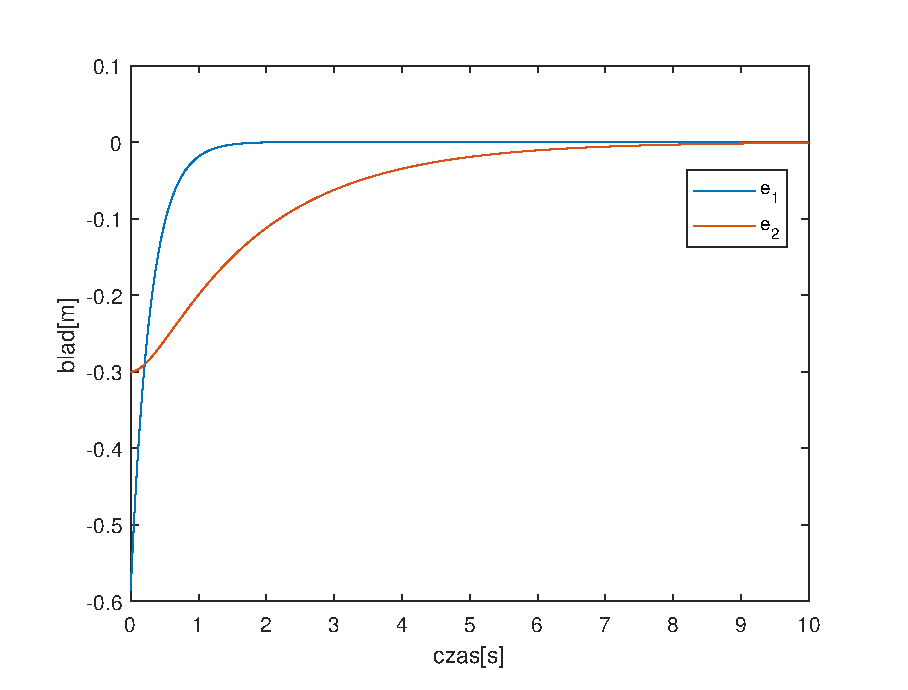
\includegraphics[width=.6\linewidth]{pics/ZPe}
\caption{Przebiegi błędów śledzenia trajektorii chwytaka}
\label{fig:ZPe}
\end{figure}

Przebiegi konfiguracji bazy i manipulatora pokazano na rys. \ref{fig:ZPq}
\begin{figure}[H]
\centering 
\begin{minipage}{.5\textwidth}
  	\centering
  	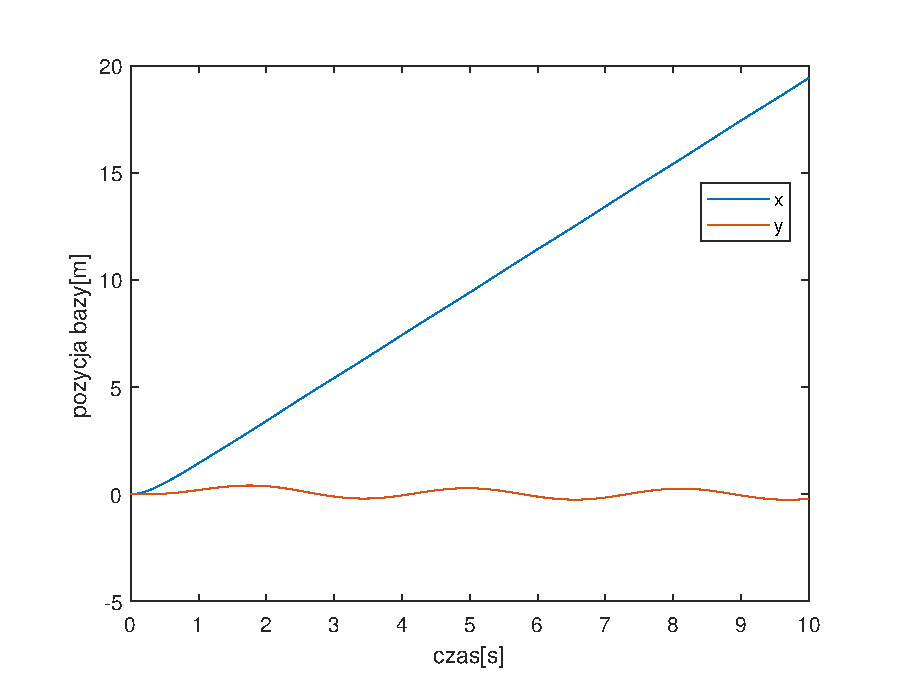
\includegraphics[width=.99\linewidth]{pics/ZPx}
  	
  	\label{fig:sub1}
\end{minipage}%
\begin{minipage}{.5\textwidth}
 	\centering
    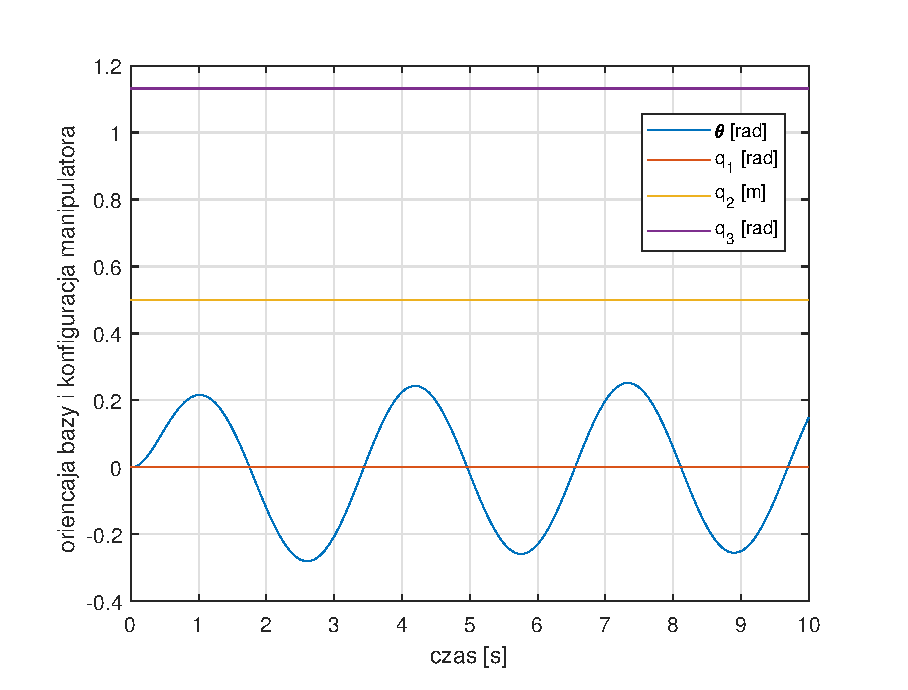
\includegraphics[width=.99\linewidth]{pics/ZPq}
 	
  	\label{fig:sub1}
\end{minipage}%
\caption{Przebiegi konfiguracji bazy i manipulatora}
\label{fig:ZPq}
\end{figure}
\section{Algorytm z rozszerzonymi funkcjami wyjściowymi}
\subsection{Specyfikacja podejścia}
Odmiennie od założeń Yamamoto i Yun'a rozszerzony algorytm nie wymaga bezruchu manipulatora. Dzięki temu platforma i manipulator mogą działać równolegle w sposób skoordynowany. Sterowanie platformy nie odbywa się w sposób bezpośredni.\\
Algorytm ten stosować można nawet wówczas, gdy np. sterowanie bazą jest niemożliwe(np. w przypadku robota free-floating).
\subsection{Funkcje wyjścia}
Funkcja wyjściowa zależy teraz od konfiguracji całego robota tj. zarówno od platformy, jak i manipulatora. Przyjmuje ona postać\cite{1}:
\begin{equation}
y(q)=\left(
\begin{array}{c}
y_1(q_m,q_r)\\
y_2(q_r)\\
\end{array}
\right),
\end{equation}
gdzie $y_1(q_m,q_r)$ jest wektorem wybranych współrzędnych efektora w podstawowym układzie odniesienia ($X_0$,$Y_0$), a $y_2(q_r)$ to wektor wybranych współrzędnych efektora w lokalnym układzie odniesienia ($X_P$,$Y_P$) związanym ze środkiem masy platformy.\\
\par Liczba współrzędnych efektora w układzie ($X_0$,$Y_0$), które można odpsprząc zależy od liczby sterowań platformą. W przypadku platformy klasy $(2,0)$ możemy śledzić dwie współrzędne.\\
\subsection{Algorytm sterowania}
\par Identycznie jak w przypadku algorytmu podstawowego, algorytm z rozszerzonymi funkcjami wyjściowymi złożony jest z dwóch pętli sprzeżenia zwrotnego\cite{1}
\begin{itemize}[noitemsep,topsep=0pt]
\item wewnętrznej pętli linearyzującej transformację wejście-stan
\item zewnętrzej pętli linearyzującej transformację wejście-wyjście
\end{itemize}
Tak jak poprzednio wewnętrzna pętla wykorzystuje prawo sterowania z rodziny algorytmów 'obliczanych momentów'
\begin{equation}
\label{eq:petla1}
u=B^{*-1}[C^*z+D^*+Q^*v].
\end{equation}
Prawo pętli wewnętrznej wyprowadzimy analogicznej jak w \ref{YYalgster}\\
Obliczmy pochodną funkcji wyjściowej $y(q)$ po czasie
\begin{equation}
\dot{y}(q)=
\left(
\begin{array}{c}
    \frac{\partial y_1}{\partial q_m} \dot{q}_m  + \frac{\partial y_1}{\partial q_r} \dot{q}_r \\
     \frac{\partial y_2}{\partial q_r} \dot{q}_r\\
\end{array}
\right)=
\begin{bmatrix}
    \frac{\partial y_1}{\partial q_m} G_m(q_m)     & \frac{\partial y_1}{\partial q_r}  \\
    0       & \frac{\partial y_2}{\partial q_r} \\
\end{bmatrix}
\left(
\begin{array}{c}
\eta\\
\dot{q}_r\\
\end{array}
\right)=\Phi(q)z,
\end{equation} 
\[
\Phi(q)=
\begin{bmatrix}
    \frac{\partial y_1}{\partial q_m} G_m(q_m)      & \frac{\partial y_1}{\partial q_r}  \\
    0       & \frac{\partial y_2}{\partial q_r} \\
\end{bmatrix}=
\begin{bmatrix}
    \Phi_m       & \Phi_{mr} \\
    0       & \Phi_r  \\
\end{bmatrix}.
\]
Ponownie zróżniczkujmy $\dot{y}(q)$ po czasie
\begin{equation}
\label{eq:1}
\ddot{y}(q,\dot{q})=\dot{\Phi}(q,\dot{q})z+\Phi(q) \dot{z}.
\end{equation} 
Stosując pierwszą pętlę (\ref{eq:petla1}) do modelu (\ref{modelpp}) otrzymamy
\begin{equation}
\label{eq:2}
\dot{z}=v.
\end{equation}
Po podstawieniu zależności (\ref{eq:2}) do równania (\ref{eq:1}) uzyskamy:
\begin{equation}
\ddot{y}(q,\dot{q})=\dot{\Phi}(q,\dot{q})z+\Phi(q) v.
\end{equation} 
Aby zapewnić linearyzację wejściowo-wyjściową należy więc użyć następującej pętli zewnętrznej
\begin{equation}
v=\Phi^{-1}(q)[-\dot{\Phi}(q,\dot{q}) z+\zeta].
\end{equation}
Po zastosowaniu algorytmu otrzymamy funkcję wyjściową o liniowej postaci
\begin{equation}
\ddot{y}(q,\dot{q})=\zeta.
\end{equation}
Otrzymaliśmy system identyczny jak ten po zastosowaniu algorytmu Yamamoto i Yun'a i również można nim sterować używając regulatora PD z korekcją(\ref{PD}).
\paragraph{Warunki działania algorytmu} Tak jak w przypadku podstawowego algorytmu Yamamoto i Yun'a należy zapewnić odwracalość macierzy $\Phi$. Warunek taki trzeba spełnić aby algorytm funkcjonował. Ma on następującą postać
\begin{equation}
\text{det}(\Phi)=\text{det}(\Phi_m)\text{det}(\Phi_r)\neq0
\end{equation}
\subsection{Badania symulacyjne}
Rozważany monocykl posiada dwa wejścia (sterowania obu kół), można więc odsprząc dwie współrzędne efektora.\\
Podczas badań odsprzęgnięto współrzędne $x$ i $y$ efektora w podstawowym układzie odniesienia ($X_0$,$Y_0$). Funkcja wyjścia $y_1(q_m,q_r)$ ma postać\\
\begin{center}
$y_1(q_m,q_r)=
\left(
\begin{array}{c}
    x + ac_0 + l_2c_{01} + l_3c_{01}c_3 \\
    y + as_0 + l_2s_{01} + l_3s_{01}c_3\\
\end{array}
\right).$
\end{center}
Funkcja $y_2(q_r)$ to wektor współrzędnych $x$, $y$ i $z$ efektora w układzie środka masy platformy ($X_P$,$Y_P$)\\
\begin{center}
$y_2(q_r)=
\left(
\begin{array}{c}
     a + l_2c_{1} + l_3c_{1}c_3 \\
     l_2s_{1} + l_3s_{1}c_3\\
     s_3l_3+q_2
\end{array}
\right).$
\end{center}
Parametry geometryczne ustalono jako: $l_2=0.3$m, $l_3=0.2$m, $a=0.2$m.\\
Początkowe położenie platformy było równe $q_m(0)=(x(0),y(0),\theta(0),\phi_1(0),\phi_2(0))=(0,0,0,0,0)$, a początkowa konfiguracja manipulatora była równa $q_r(0)=(q_1(0),q_2(0),q_3(0))=(\frac{\pi}{2},0.2,-\frac{\pi}{2})$.\\
Prędkości początkowe $\dot{q}(0)$ były równe zeru.  \\
Funkcje wyjściowe miały następujące wartości początkowe 
\begin{center}
$y(q_m(0),q_r(0))=
\left(
\begin{array}{c}
    0.2 \\
     0.3 \\
      0.2 \\
     0.3 \\
     0 \\
\end{array}
\right).$
\end{center}
Wektor pochodnych $\dot{y}$ był zerowy.\\
Wybrano następujące trajektorie zadane $y_d(t)$ 
\begin{center}
$y_d(t)=
\left(
\begin{array}{c}
    2t\\
    -0.3\cos{(2t)}\\
    0.5\\
    -0.3\\
    0.2\\
\end{array}
\right).$
\end{center}
Błąd początkowy $e(t)=y_d(t)-y(t)$ i jego pochodna były równe
\begin{center}
$e(0)=
\left(
\begin{array}{c}
   -0.2\\
    -0.6\\
    0.3\\
    -0.6\\
    0.2\\
\end{array}
\right), \hspace{1.5cm}
\dot{e}(0)=
\left(
\begin{array}{c}
    2\\
    0\\
    0\\
    0\\
    0\\
\end{array}
\right).$
\end{center}
Do sterowania układem liniowym użyto regulator PD z korektą (\ref{PD}) z nastawami $K_d=4$, $K_p=2$.
W badaniach wykorzystano środowisko Matlab/Simulink. \\

\begin{figure}[H]
\centering
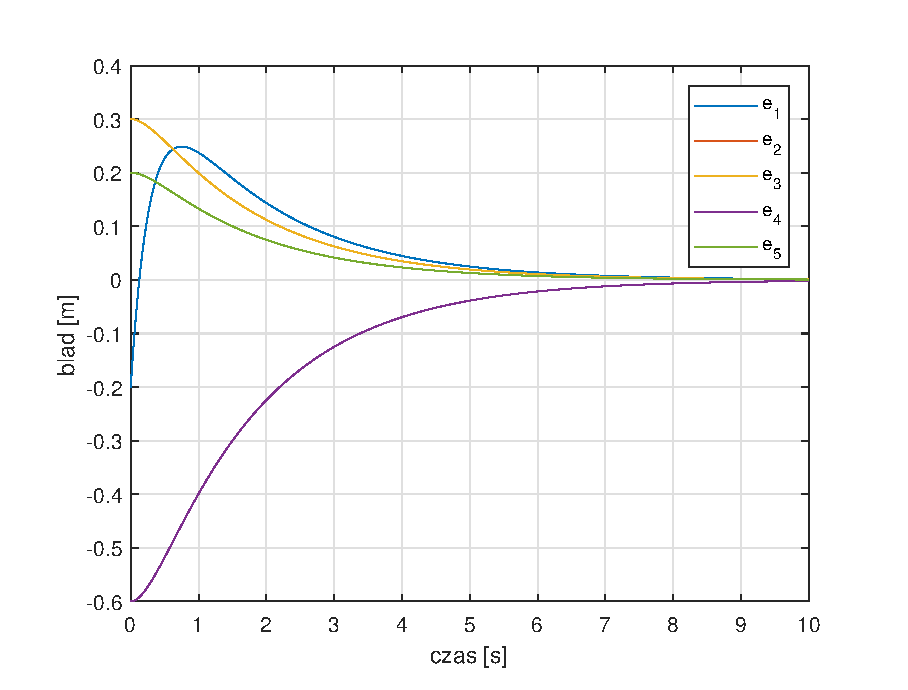
\includegraphics[width=.6\linewidth]{pics/ZRe}
\caption{Przebieg błędu}
\label{fig:regnad}
\end{figure}

\begin{figure}[H]
\centering 
\begin{minipage}{.5\textwidth}
  	\centering
  	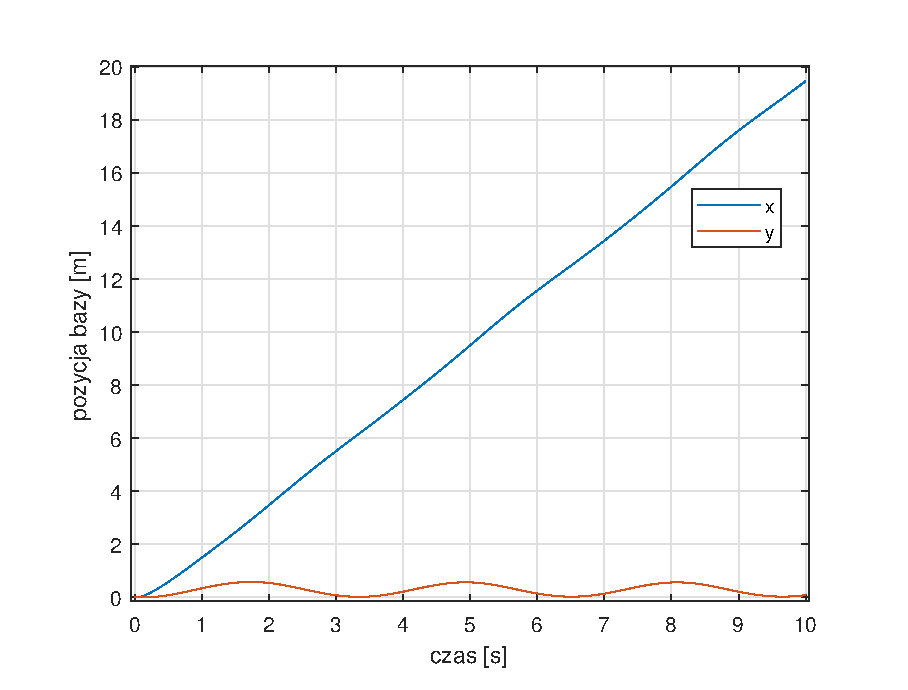
\includegraphics[width=.99\linewidth]{pics/ZRx}
  	
  	\label{fig:sub1}
\end{minipage}%
\begin{minipage}{.5\textwidth}
 	\centering
    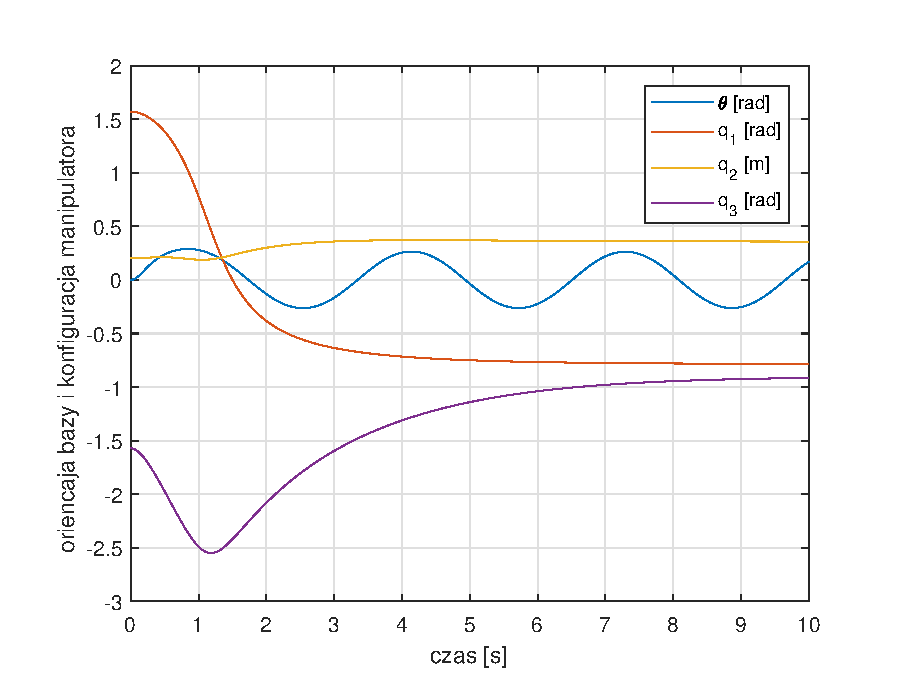
\includegraphics[width=.99\linewidth]{pics/ZRq}
 	
  	\label{fig:sub1}
\end{minipage}%
\caption{Przebieg konfiguracji bazy i manipulatora}
\label{fig:regnad}
\end{figure}
\chapter{Model satelity typu free-floating}
\chapter{Odsprzęganie wejściowo-wyjściowe dla satelity typu free-floating}
\begin{thebibliography}{99}
\bibitem{1} Mazur A. \textit{New approach to designing input-output decoupling controllers for mobile manipulators}. Bull. of the Polish Academy of sciences Tech. Sci. 53(1):31-37, (2005)

\bibitem{2} Yamamoto Y, Yun X. \textit{Coordinating locomotion and manipulation of a mobile manipulator.} IEEE Trans. on Automatic Control, 39(6):1326-1332, (1994)

\bibitem{3} Yamamoto Y, Yun X. \textit{Effect of the dynamic interaction on coordinated control of mobile manipulators.} IEEE Trans. Robotics Automat, 12(5):816-824, (1996)

\bibitem{4} Mazur A, Arent K. \textit{Lecture Notes in Control and Information Sciences}, 335:55-71 (2007)

\bibitem{5} Tchoń K, Jakubiak J. \textit{Acceleration-Driven Kinematics of Mobile Manipulators: An Endogenous Configuration Space Approach}, pp.(469-476),  (2004)

\bibitem{6} M. R. Flannery. \textit{The Enigma of Nonholonomic Constraints.} American Association of Physics Teachers, 73(3):265–272, (2005).

\bibitem{7} Yamamoto Y, Yun X. \textit{Coordinating locomotion and manipulation of a mobile manipulator.} In Proceedings of 31st IEEE Conference on Decision and Control, pp.(2643-2648), (1992)
\end{thebibliography}

%\addcontentsline{toc}{chapter}{Bibliografia}
\begin{thebibliography}{10}
\bibitem{AlSa16} A. Salwach, "Wizualizacja i analiza robotyczna postury bramkarza sportowego", inżynierska praca dyplomowa, Wydział
  Elektroniki, Politechnika Wrocławska 2016.  
\bibitem{Kinect} http://www.xbox.com/en-US/xbox-one/accessories/kinect
\bibitem{game} J. D. Williams, "Strateg doskonały. Wprowadzenie do teorii gier", PWN, Warszawa 1965
\bibitem{game2} http://www.fuw.edu.pl/\textasciitilde kostecki/teoria\underline{\hspace{.1in}}gier.pdf
\bibitem{MSpong} M. Spong, M. Vidyasagar, "Dynamika i sterowanie robotów", WNT, Warszawa 1997
\bibitem{Eigen} http://eigen.tuxfamily.org/
\bibitem{rapidXml} http://rapidxml.sourceforge.net/
\bibitem{doxygen} http://www.stack.nl/\textasciitilde dimitri/doxygen/
\bibitem{qt} https://www.qt.io/qt5-7/
\bibitem{body} R. Contini, "Body Segment Parametsrs, Part II", \textit{Artificial Limbs}, Washington D.C. 1972
\bibitem{Wolfram} C. Hastings, K. Mischo, M. Morrison, "Hands-On Start to Wolfram Mathematica", Wolfram Media, Inc. 2015
\bibitem{multiresgrid} R. D. Jovanović, M. Tuba, D. Simian, "An Algorithm for
  Multi-Resolution Grid Creation Applied to Explicit Finite Difference Scheme",
  Proc.\  of the 12th WSEAS Int.\ Conf.\ on COMPUTERS 2008. 
\end{thebibliography}




%\bibliography{bibliografia} % bibliografia.bib

%opcjonalnie może się tu pojawić spis rysunków i tabel
% \listoffigures
% \listoftables
\end{document}
